A program that runs on GPU is called \textit{shader}. Shaders are principally used to modify the representation and the behaviour of 3D objects. They are also used to create lighting effects.  Shaders can perform tasks efficiently thanks to the GPU. That guarantee faster results than CPU since GPU is designed to work in parallel.
These shader programs are written in \textit{GLSL}.

\section{GPU pipeline}
Using a program will allow us to control the rendering pipeline, by default there is no pipeline set in OpenGL. We pass a set of vertices as input, then the \textit{vertex shader} transforms them (translation, rotation, projection...) and passes the transformed vertices to the \textit{geometry shader}. This shader takes vertices to create primitive shapes and then it rasterizes them. These rasterized flat images are then passed as input to the \textit{fragment shader} that adds the lighting, apply textures and color these images (Fig. \ref{fig:gpu-pipeline}).

\begin{figure}
    \scalebox{0.85}{\begin{tikzpicture}
        [node distance=.8cm,
        start chain=going right,]
        \node[punktchain, join] (vs) {Vertex Shader};
        \node[punktchain, join] (gs)  {Geometry Shader};
        \node[punktchain, join] (fs)  {Fragment Shader};
    \end{tikzpicture}} \\ \\
    \scalebox{0.9}{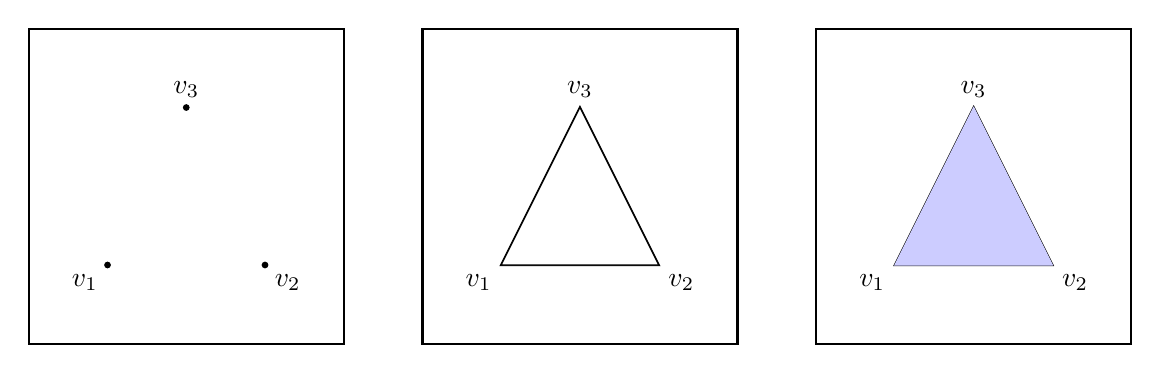
\begin{tikzpicture}
        \coordinate (L1) at (6,0);
        \coordinate (L2) at (8,0);
        \coordinate (L3) at (7,2);

        \coordinate (S1) at (5,-1);
        \coordinate (S2) at (9,-1);
        \coordinate (S3) at (5,3);
        \coordinate (S4) at (9,3);

        \draw[thick] (S1) --  (S2)
                        --  (S4)
                        --  (S3)
                        --  (S1) -- cycle;


        \coordinate (L11) at (11,0);
        \coordinate (L12) at (13,0);
        \coordinate (L13) at (12,2);

        \coordinate (S11) at (10,-1);
        \coordinate (S12) at (14,-1);
        \coordinate (S13) at (10,3);
        \coordinate (S14) at (14,3);


        \draw[thick] (L11) -- (L12)
                        -- (L13)
                        -- (L11) -- cycle;

        \draw[thick] (S11) --  (S12)
                        --  (S14)
                        --  (S13)
                        --  (S11) -- cycle;

        %%%
        \coordinate (L21) at (16,0);
        \coordinate (L22) at (18,0);
        \coordinate (L23) at (17,2);

        \coordinate (S21) at (15,-1);
        \coordinate (S22) at (19,-1);
        \coordinate (S23) at (15,3);
        \coordinate (S24) at (19,3);


        \draw[thick] (L21) -- (L22)
                        -- (L23)
                        -- (L21) -- cycle;

        \draw[thick] (S21) --  (S22)
                        --  (S24)
                        --  (S23)
                        --  (S21) -- cycle;
        \filldraw[draw=black, fill=white] (L11) -- (L12) -- (L13) -- cycle;
        \filldraw[draw=blue!20, fill=blue!20] (L21) -- (L22) -- (L23) -- cycle;
        \draw (L1) node [below left] {$v_1$}
            (L2) node [below right] {$v_2$}
            (L3) node [above] {$v_3$};
        \filldraw (6,0) circle (1pt);
        \filldraw (8,0) circle (1pt);
        \filldraw (7,2) circle (1pt);

        \draw (L11) node [below left] {$v_1$}
            (L12) node [below right] {$v_2$}
            (L13) node [above] {$v_3$};

        \draw (L21) node [below left] {$v_1$}
            (L22) node [below right] {$v_2$}
            (L23) node [above] {$v_3$};
    \end{tikzpicture}}
    \caption{GPU pipeline} \label{fig:gpu-pipeline}
\end{figure}


\section{Vertex Shader}
The program that perform vertex operations is called \textit{vertex shader}. It receives one vertex at a time and then it passes the output to a \textit{fragment shader} or to a \textit{geometry shader}, if any.

\section{Fragment Shader}
\textit{Fragment shader} performs color computation for every visible pixel of the rasterized object. It works on a fragment at a time, but thanks to the power of GPU it can work in parallel for all vertices (\textit{vertex shader}) and fragments (\textit{fragment shader}).

\section{Geometry Shader}
\textit{Geometry shader} is used for layered rendering. It takes as input a set of vertices (single primitive, example: triangle or a point) and it transforms them before sending to the next shader stage. In this way, we can obtain different primitives.

Each time we call the function \texttt{EmitVertex()} the vector currently set to \texttt{gl\_Position} is added to the primitive. All emitted vertices are combined for the primitive and output when we call the function \texttt{EndPrimitive()}.